\section{Miniaturized Broadband Antenna Loaded With Frequency Selective Surface for Corona Discharge Detection}

\subsection*{Contexto y objetivo}
La descarga de corona es un fenómeno común en líneas de transmisión de alto voltaje, que provoca daños en el aislamiento y pérdidas de energía. Los métodos de detección actuales, como las antenas, tienen una sensibilidad limitada que impide la identificación precisa de la ubicación de las descargas. Los diseños de antenas existentes son a menudo grandes (e.g., 2x4 m o 360 mm de diámetro) y solo pueden detectar la presencia o ausencia de corona, sin determinar la ubicación exacta, lo que limita su uso con vehículos aéreos no tripulados (UAV). Trabajos previos han demostrado que la superposición de una Superficie Selectiva en Frecuencia (FSS) en una antena puede mejorar su capacidad para capturar ondas electromagnéticas.

El objetivo principal de este estudio es diseñar una FSS miniaturizada de banda ancha que opere en el rango de frecuencia de descarga de corona (100–500 MHz) para mejorar la sensibilidad y la distancia de detección de las antenas, permitiendo una detección más precisa y segura de las descargas de corona, especialmente para aplicaciones con UAVs.

\subsection*{Metodología o desarrollo}
El estudio se dividió en varias fases: diseño de la FSS, simulación de la antena y experimentos de detección de descarga de corona.

\textbf{1. Diseño de la Superficie Selectiva en Frecuencia (FSS):}
\begin{itemize}
    \item \textbf{Requisitos de diseño:} La FSS fue diseñada para operar entre 100 y 500 MHz, donde la energía de la señal de descarga de corona es más pronunciada y el ruido es bajo. Se requirió un valor de S11 < -10 dB para absorber más del 90\% de la onda electromagnética incidente y un tamaño de celda pequeño para evitar lóbulos de rejilla.
    \item \textbf{Evolución de la celda FSS:} El diseño comenzó con una celda cruzada básica, la cual fue mejorada al doblar y extender los extremos de los cuatro brazos en ángulos de 90° para formar una estructura serpentina. Esta evolución gradual, como se muestra en la Figura \ref{fig:fss_evolution}, buscó reducir la frecuencia resonante.
    \begin{figure}[htpb]
    \centering
    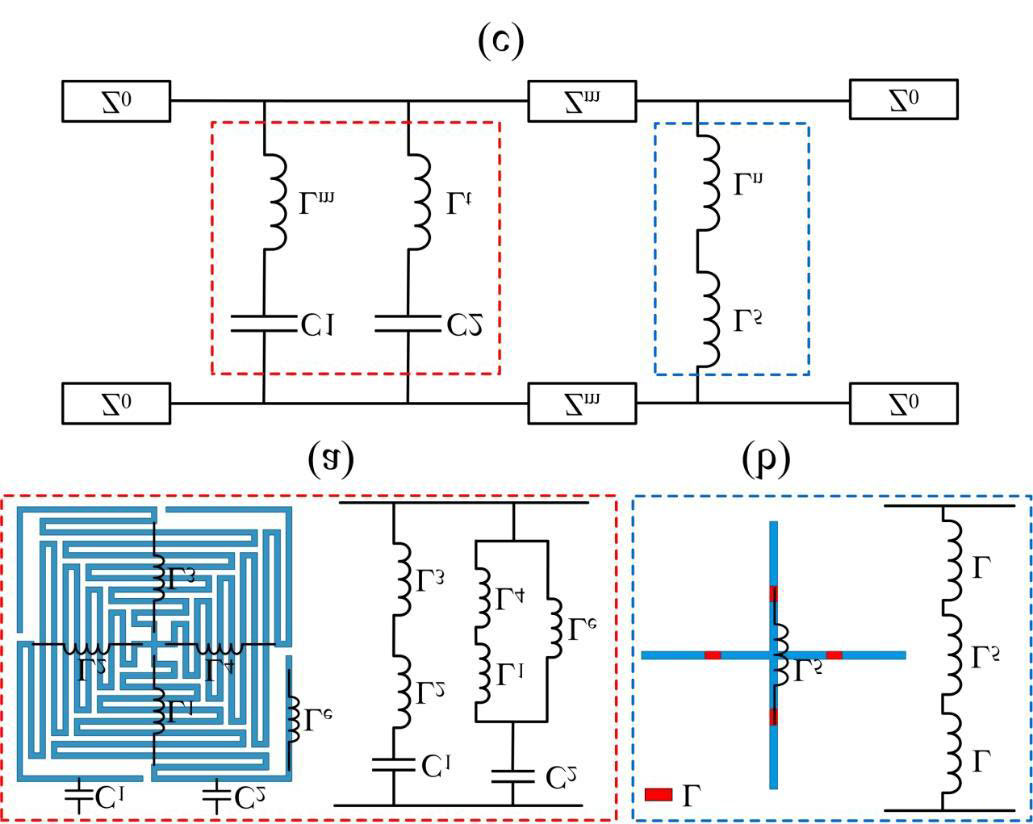
\includegraphics[width=0.8\textwidth]{images/564630268a062c85fb92b70f0c2f667c_p3_i1.jpeg}
    \caption{Proceso de conversión de la FSS de capa única de señal.}
    \end{figure}
    \item \textbf{Diseño de doble capa:} Se añadió un parche metálico en la parte posterior del sustrato dieléctrico para formar una FSS de doble capa, con la parte inferior con componentes inductivos para reducir aún más la frecuencia resonante. La celda FSS final (Figura \ref{fig:final_fss}) tiene dimensiones de 10 x 10 x 1.6 mm.
    \begin{figure}[htpb]
    \centering
    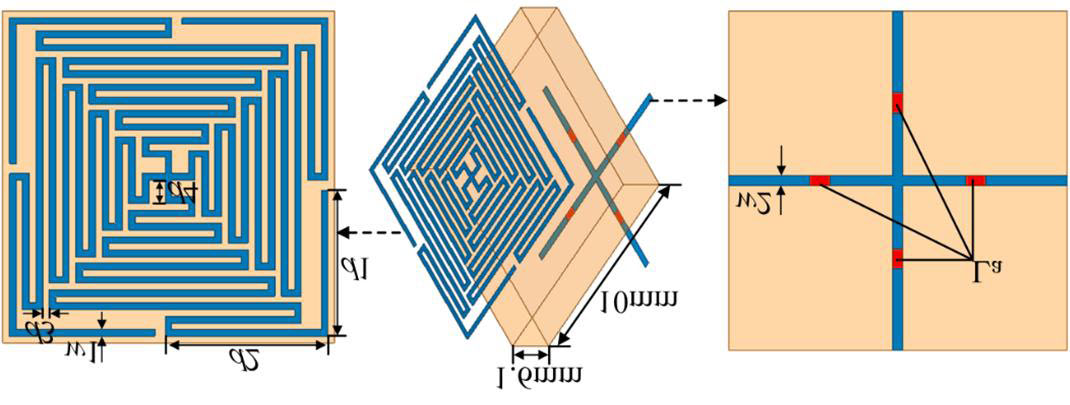
\includegraphics[width=0.8\textwidth]{images/564630268a062c85fb92b70f0c2f667c_p4_i5.jpeg}
    \caption{Estructura general de la FSS finalizada.}
    \end{figure}
    \item \textbf{Circuito equivalente:} Se construyó un circuito equivalente para analizar el comportamiento de la FSS (Figura \ref{fig:equivalent_circuit}), identificando capacitores (C1, C2) y bobinas (L1, L2, L3, L4, Lm, Ln, Ls) basadas en la distribución del campo eléctrico y la corriente superficial.
    \begin{figure}[htpb]
    \centering
    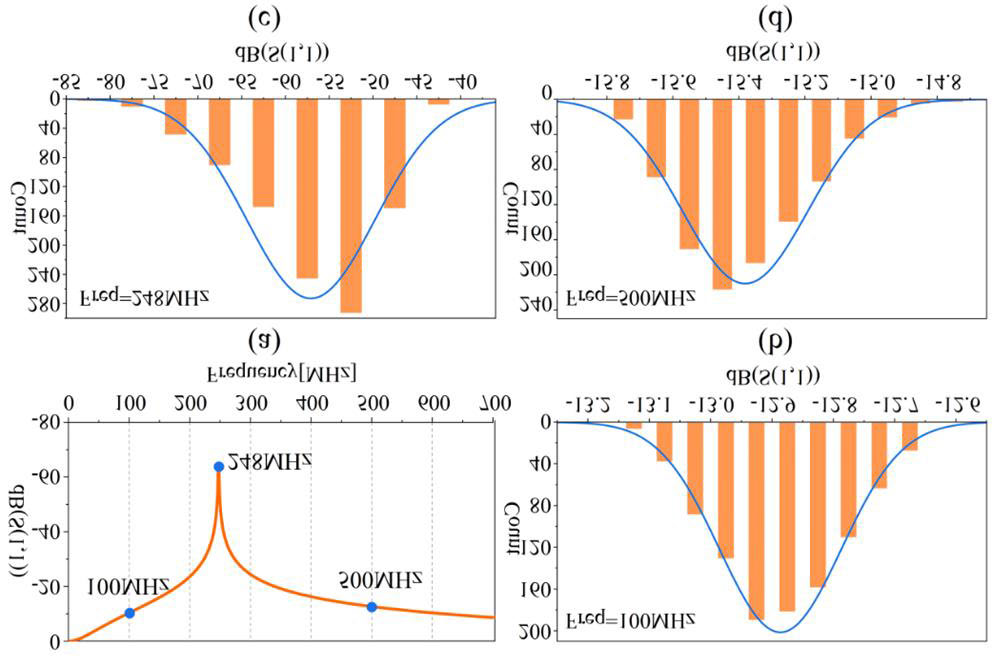
\includegraphics[width=0.8\textwidth]{images/564630268a062c85fb92b70f0c2f667c_p4_i1.jpeg}
    \caption{(a) Circuito equivalente del parche metálico superior. (b) Celda cruzada y circuito equivalente del inductor de chip cargado. (c) Circuito equivalente finalizado.}
    \end{figure}
    \item \textbf{Análisis de Monte Carlo:} Se realizó un análisis de Monte Carlo utilizando ANSYS para evaluar el impacto de las tolerancias de ±5\% en el valor de la inductancia del chip (390 nH nominal) en el rendimiento S11 de la FSS.
\end{itemize}

\textbf{2. Simulación y Análisis de Antenas:}
\begin{itemize}
    \item \textbf{Antena de detección:} Se utilizó una antena fractal de Hilbert serpentina (SHU) preexistente de 130 × 130 × 1.6 mm como antena de detección.
    \item \textbf{Superposición de FSS:} La FSS diseñada se colocó sobre la antena SHU (formando la antena FSHU), y se simuló la distancia óptima 'h' entre la FSS y la antena. Se probaron alturas de 10, 20, 30 y 40 mm. El principio de operación se muestra en la Figura \ref{fig:fss_principle}.
    \begin{figure}[htpb]
    \centering
    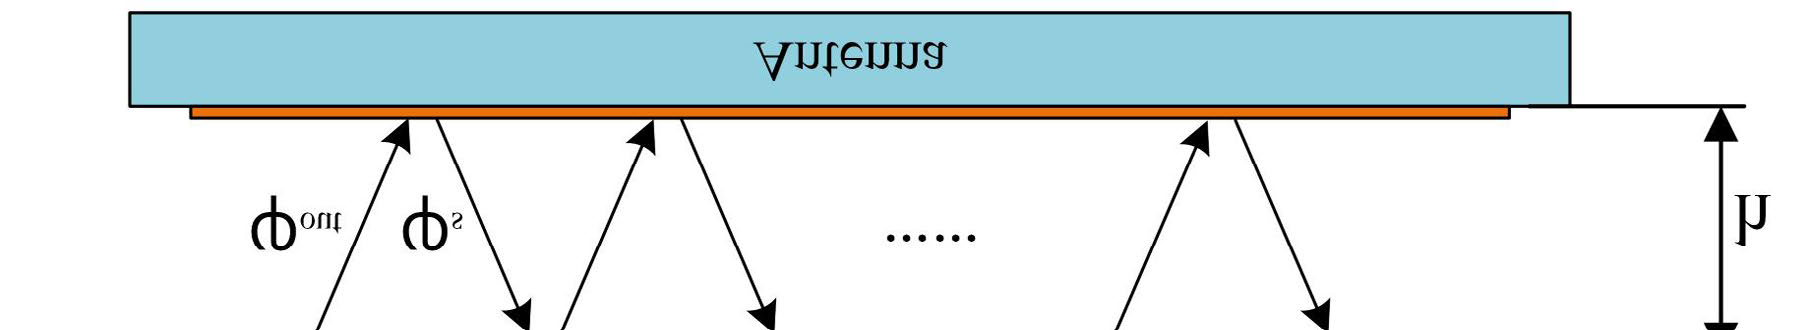
\includegraphics[width=0.8\textwidth]{images/564630268a062c85fb92b70f0c2f667c_p2_i3.jpeg}
    \caption{Principio de funcionamiento de la matriz FSS en antenas apiladas.}
    \end{figure}
    \item \textbf{Configuración de límites:} Se utilizaron configuraciones de límites específicas en las simulaciones (puertos floquet, límites maestro-esclavo) para la FSS y límites radiantes para la antena FSHU.
\end{itemize}

\textbf{3. Experimentos de Detección de Descarga de Corona:}
\begin{itemize}
    \item \textbf{Fabricación:} Se fabricaron prototipos de la antena SHU y la matriz FSS utilizando tecnología PCB estándar y técnicas de colocación de máquinas (Figura \ref{fig:fabricated_antennas}).
    \begin{figure}[htpb]
    \centering
    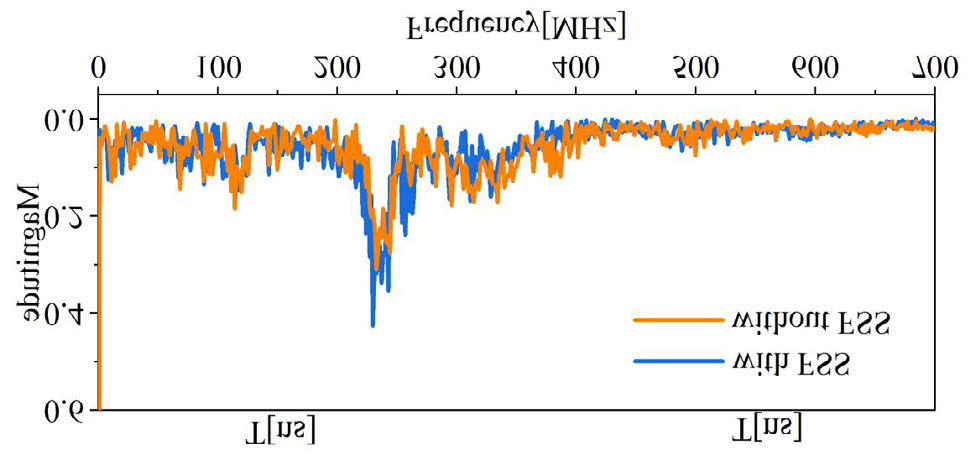
\includegraphics[width=0.8\textwidth]{images/564630268a062c85fb92b70f0c2f667c_p7_i2.jpeg}
    \caption{(c) Antena SHU física. (d) Comparación de la curva S11 medida con la simulación.}
    \end{figure}
    \item \textbf{Plataforma experimental:} Se montó una plataforma de prueba (Figura \ref{fig:experimental_platform}) que incluía un sistema transformador de 10 kA/50 kV, aisladores compuestos con contaminación artificial, las antenas SHU y FSHU, filtros de paso de banda (100-500 MHz), un amplificador de bajo ruido (LNA) y un osciloscopio multicanal (RIGOL MSO2202A).
    \begin{figure}[htpb]
    \centering
    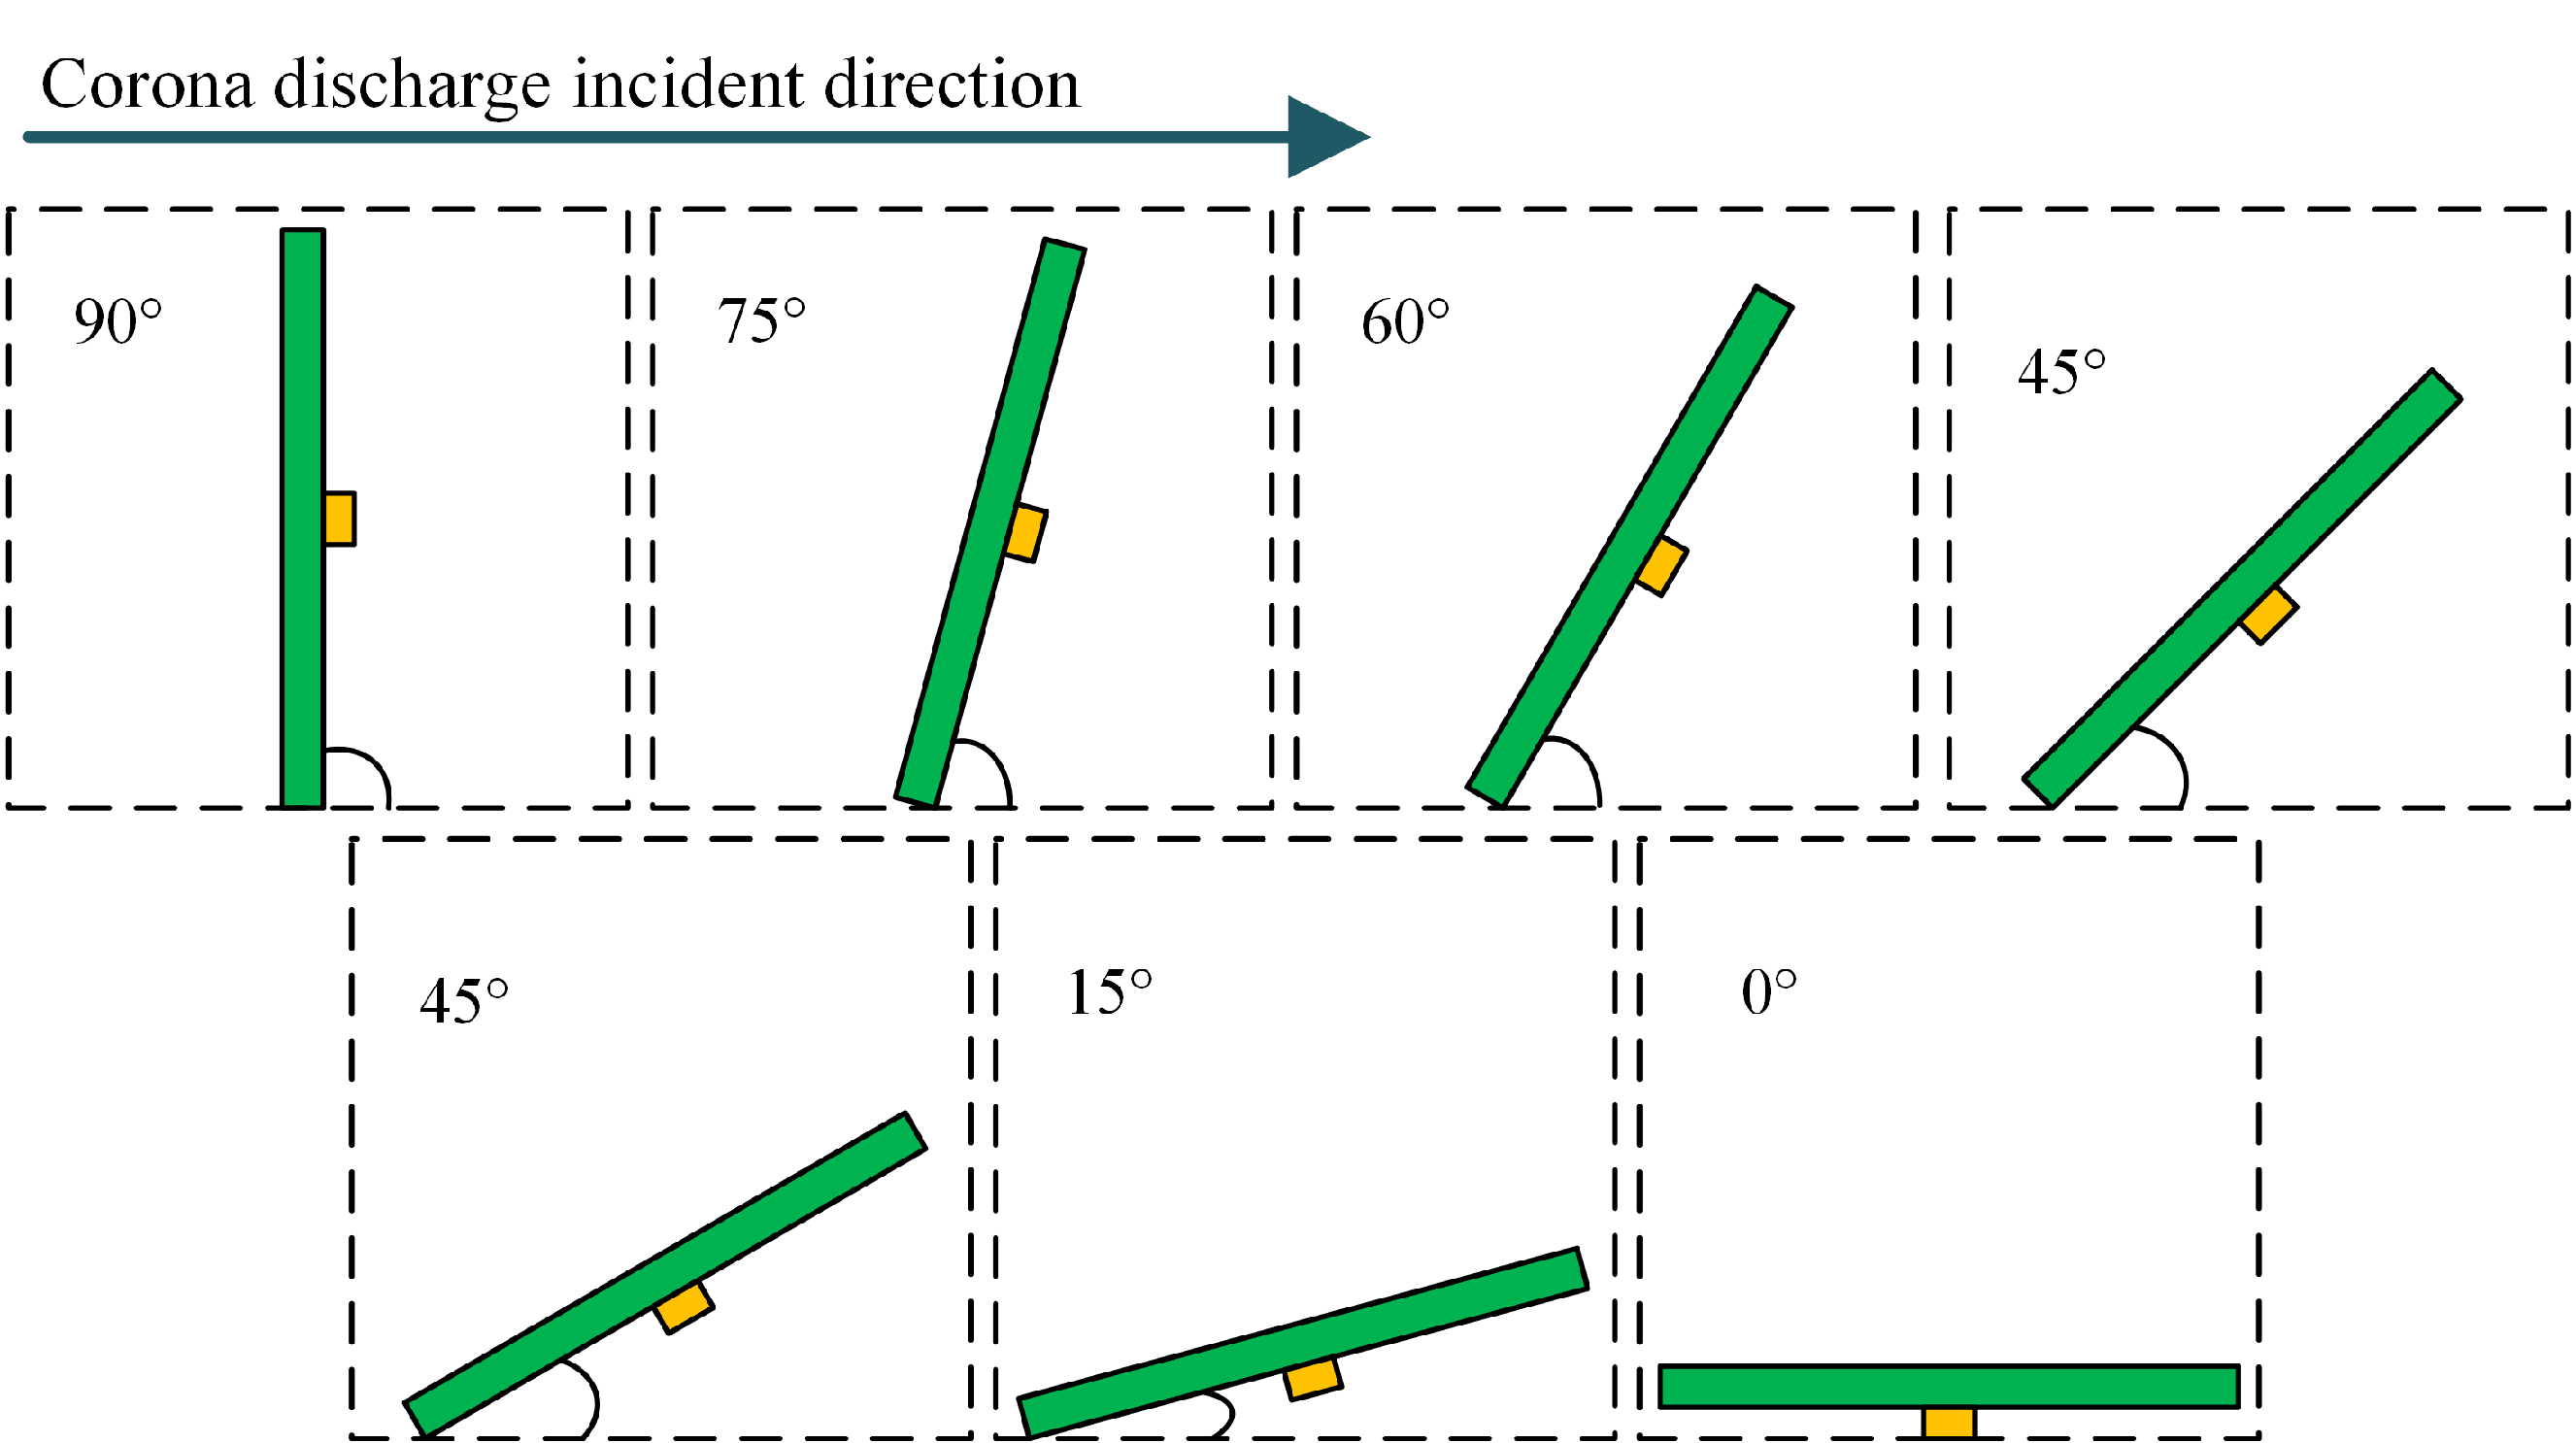
\includegraphics[width=0.8\textwidth]{images/564630268a062c85fb92b70f0c2f667c_p7_i1.png}
    \caption{Plataforma experimental.}
    \end{figure}
    \item \textbf{Pruebas de detección:} Se detectaron señales de descarga de corona a distancias de 1, 4, 7, 10 y 13 m, y también se varió el ángulo de colocación de la antena (0° a 90° en incrementos de 15°) para evaluar el efecto de la dirección de la onda incidente (Figura \ref{fig:placement_angle}).
    \begin{figure}[htpb]
    \centering
    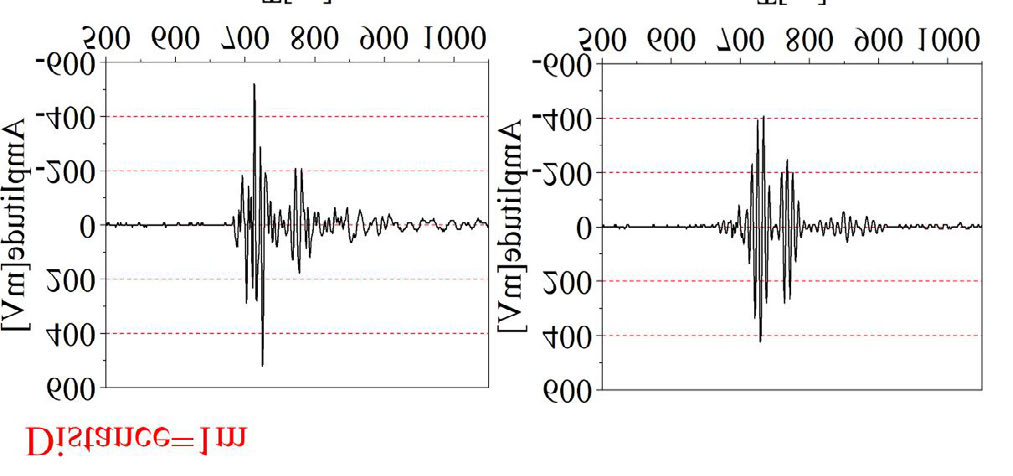
\includegraphics[width=0.8\textwidth]{images/564630268a062c85fb92b70f0c2f667c_p7_i10.jpeg}
    \caption{Esquemático del cambio del ángulo de colocación de la antena.}
    \end{figure}
    \item \textbf{Medición de carga:} Se utilizó una bobina de Rogowski de alta frecuencia para medir la capacidad de carga liberada por el circuito experimental.
\end{itemize}

\subsection*{Resultados o hallazgos}

\textbf{1. Rendimiento de la FSS:}
\begin{itemize}
    \item La FSS diseñada mostró una curva S11 < -10 dB en el rango de frecuencia de 100–500 MHz (Figura \ref{fig:fss_s11_final}), con una frecuencia resonante de 248 MHz. Esto indica una absorción de más del 90\% de la onda electromagnética en la banda de interés.
    \begin{figure}[htpb]
    \centering
    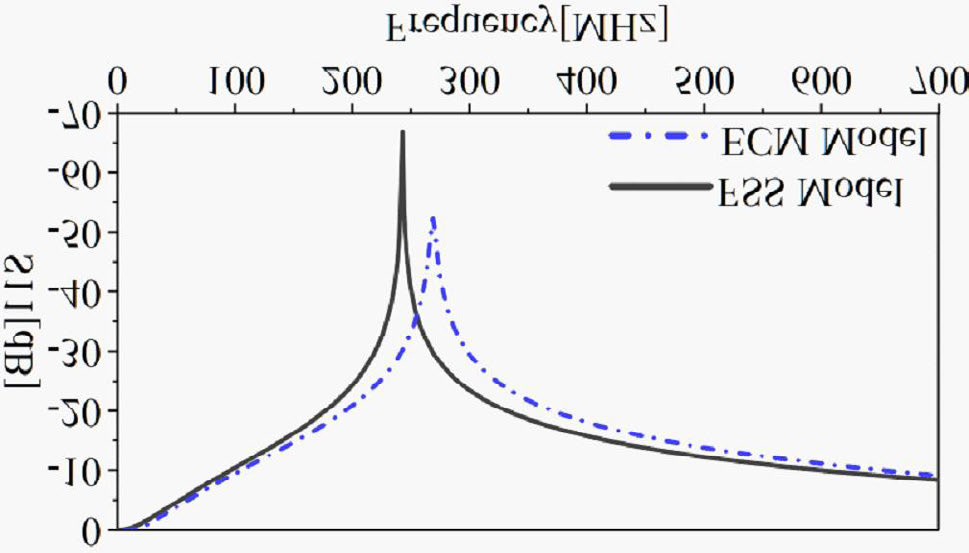
\includegraphics[width=0.8\textwidth]{images/564630268a062c85fb92b70f0c2f667c_p4_i4.jpeg}
    \caption{(c) Curva S11 de la FSS de doble capa con inductores de chip y su circuito equivalente.}
    \end{figure}
    \item El análisis de Monte Carlo (Figura \ref{fig:monte_carlo_s11}) reveló que la tolerancia del inductor afecta significativamente el parámetro S11 de la FSS a 248 MHz, pero el impacto es menor a 100 y 500 MHz, lo que confirma su influencia en la frecuencia resonante.
    \begin{figure}[htpb]
    \centering
    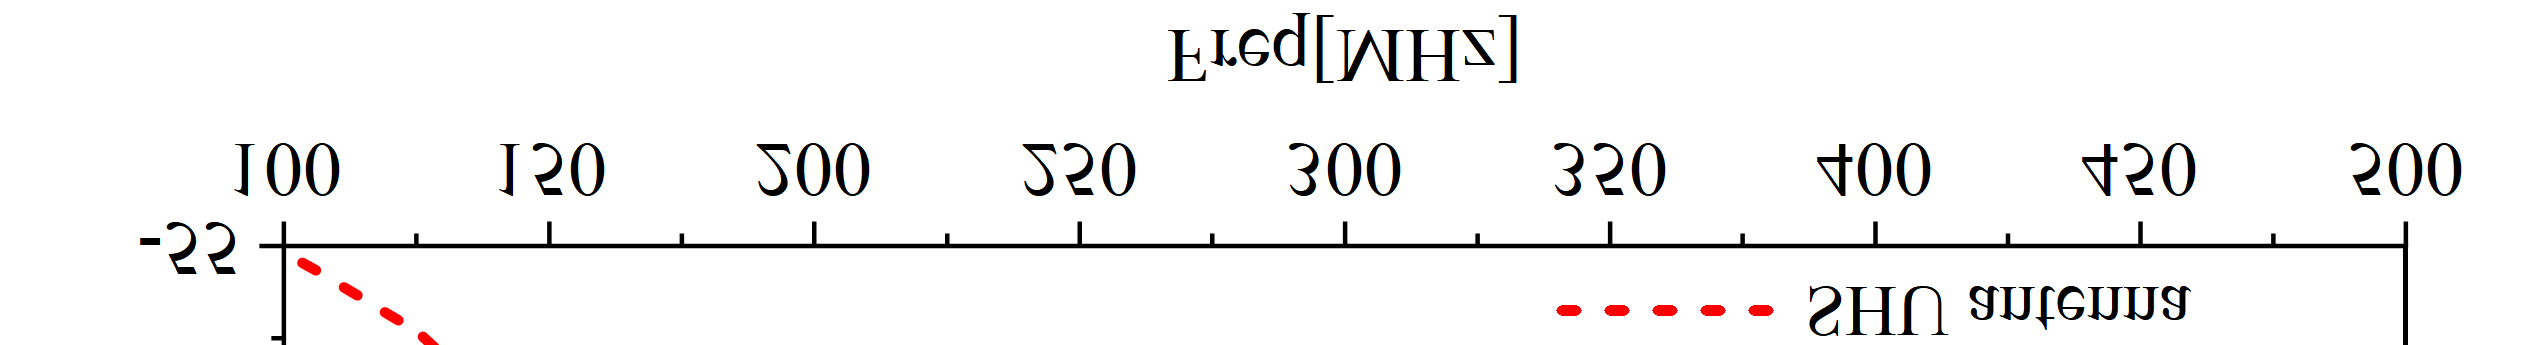
\includegraphics[width=0.8\textwidth]{images/564630268a062c85fb92b70f0c2f667c_p5_i1.png}
    \caption{(a) Curva S11 de la FSS. (b) Histograma de la distribución S11 a 100 MHz. (c) Histograma de la distribución S11 a 248 MHz. (d) Histograma de la distribución S11 a 500 MHz.}
    \end{figure}
\end{itemize}

\textbf{2. Rendimiento de la antena FSHU (FSS-SHU):}
\begin{itemize}
    \item \textbf{Distancia óptima (h):} La simulación mostró que la FSS puede mejorar la capacidad de la antena para recibir ondas electromagnéticas, siendo óptima una distancia 'h' de 20 mm entre la FSS y la antena SHU. A esta altura, la curva S11 de la antena FSHU es significativamente más baja que la de la antena SHU (Figura \ref{fig:fshu_s11_heights}), y la ganancia de la antena se maximiza (Figura \ref{fig:gain_comparison}).
    \begin{figure}[htpb]
    \centering
    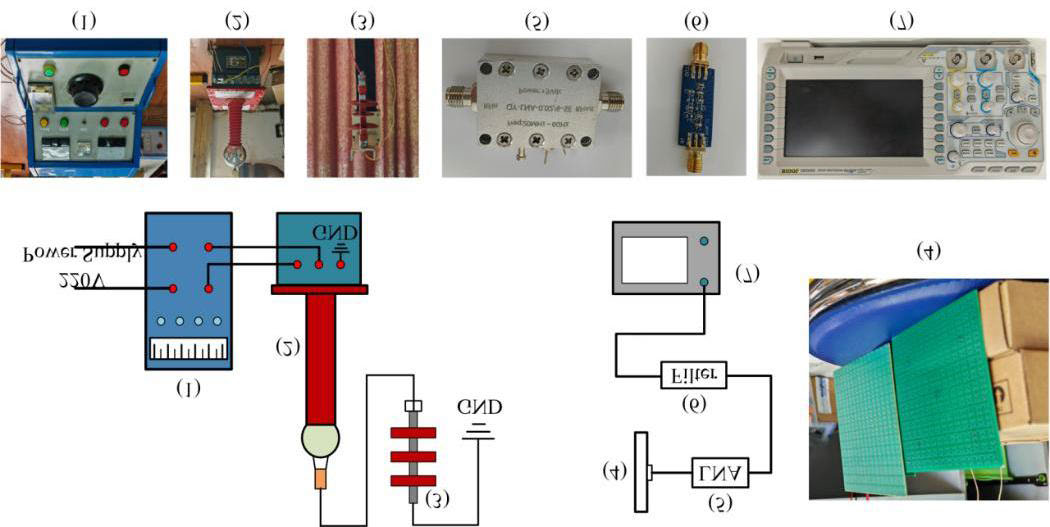
\includegraphics[width=0.8\textwidth]{images/564630268a062c85fb92b70f0c2f667c_p6_i1.jpeg}
    \caption{Curva S11 de la antena global para diferentes alturas.}
    \end{figure}
    \begin{figure}[htpb]
    \centering
    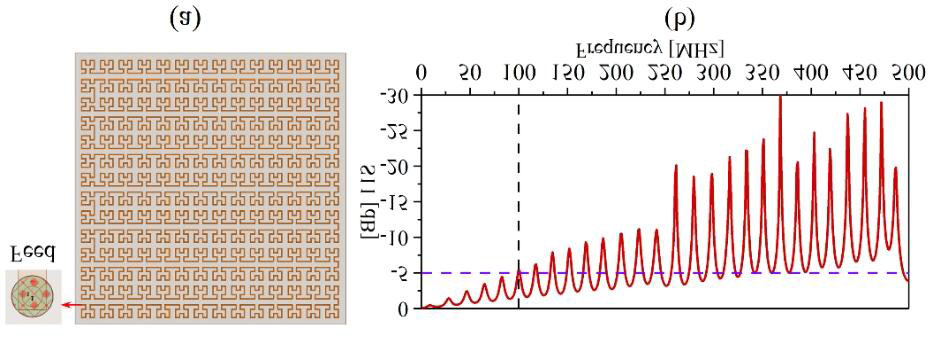
\includegraphics[width=0.8\textwidth]{images/564630268a062c85fb92b70f0c2f667c_p5_i5.png}
    \caption{Comparación de ganancia de antenas.}
    \end{figure}
    \item \textbf{Amplitud de la señal:} La antena FSHU detectó amplitudes de señal de descarga de corona 128\%, 130\%, 132\% y 135\% más altas que la antena SHU a distancias de 1, 4, 7 y 10 m, respectivamente.
    \item \textbf{Distancia máxima de detección:} La antena FSHU alcanzó una distancia máxima de detección de 13 m, donde la antena SHU ya no podía detectar la señal (Figura \ref{fig:corona_signals_distances}).
    \begin{figure}[htpb]
    \centering
    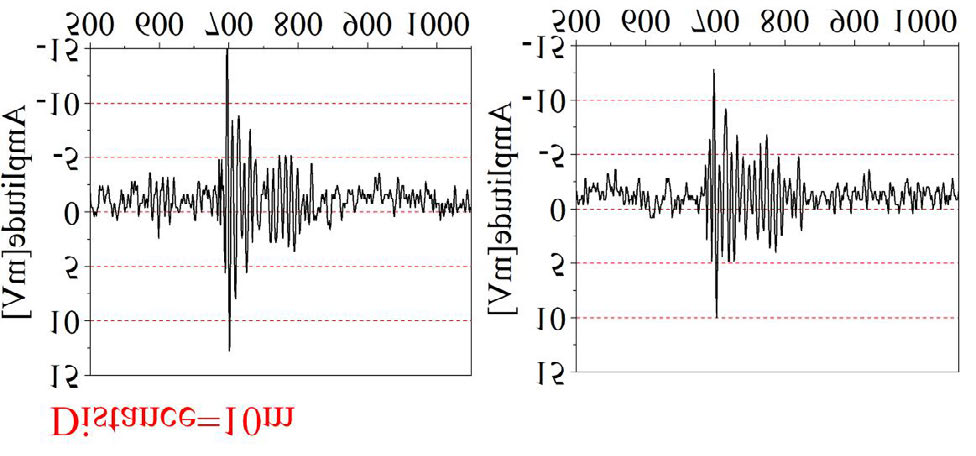
\includegraphics[width=0.8\textwidth]{images/564630268a062c85fb92b70f0c2f667c_p7_i4.jpeg}
    \caption{(a) Ruido ambiental. (b) Distancia de detección de 1 m. (c) Distancia de detección de 4 m. (d) Distancia de detección de 7 m. (e) Distancia de detección de 10 m. (f) Distancia de detección de 13 m.}
    \end{figure}
    \item \textbf{Efecto del ángulo:} La amplitud de la señal disminuyó a medida que el ángulo de incidencia se reducía. A 10 m, la FSHU no pudo detectar señales a 0°, y a 13 m, solo pudo detectar a 90° (Figura \ref{fig:amplitude_vs_angle}).
    \begin{figure}[htpb]
    \centering
    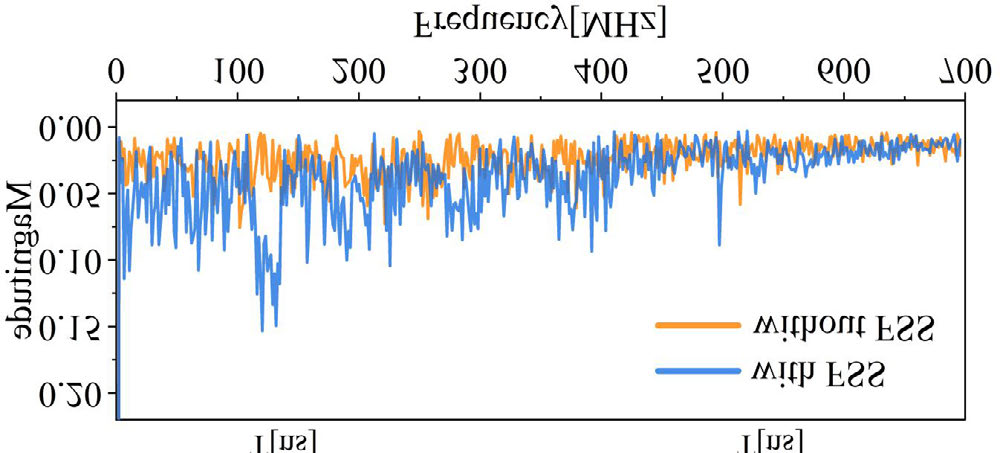
\includegraphics[width=0.8\textwidth]{images/564630268a062c85fb92b70f0c2f667c_p7_i11.jpeg}
    \caption{Amplitud promedio de la antena a diferentes distancias correspondiente al cambio en el ángulo de la antena. (a) 1 m, (b) 4 m, (c) 7 m y (d) 10 m.}
    \end{figure}
\end{itemize}

\textbf{3. Comparación con trabajos previos:}
La antena FSHU diseñada presenta una distancia de detección óptima de 13 m, superando a otras antenas en la literatura que son significativamente más grandes y menos portátiles, como se detalla en la Tabla \ref{tab:comparison_table}.

\begin{table}[htpb]
\centering
\caption{Comparación con otros trabajos}
\begin{tabular}{|c|c|c|}
\hline
\textbf{Ref. No.} & \textbf{Tamaño} & \textbf{Distancia de detección} \\
\hline
{[}7{]} & 2x4 m (superficie de recepción) & 320m \\
{[}8{]} & Diámetro: 360 mm, Altura: 2284 mm & 260m \\
{[}10{]} & 100mm$\times$100mm$\times$1.6mm & 5m \\
\textbf{Este trabajo} & \begin{tabular}{c} 130mm$\times$130mm$\times$1.6mm con \\ 150mm$\times$150mm$\times$1.6mm \end{tabular} & \textbf{13m} \\
\hline
\end{tabular}
\end{table}

\subsection*{Discusión o análisis crítico}

El principio de funcionamiento de la FSS para mejorar la sensibilidad se basa en un efecto de multicapa. La FSS, al ser una estructura electromagnética artificial compuesta de celdas periódicamente arregladas, refleja y transmite selectivamente las ondas electromagnéticas. Al superponerla sobre la antena de detección, la onda electromagnética incidente atraviesa la FSS, se convierte en una onda saliente, una parte es capturada por la antena y el resto se refleja. Esta onda reflejada incide nuevamente en la parte trasera de la FSS, que la vuelve a reflejar hacia la antena, repitiendo este ciclo. Este proceso cíclico aumenta la cantidad total de ondas electromagnéticas capturadas por la antena, mejorando su sensibilidad.

Aunque los resultados de simulación y experimentales muestran una clara mejora en la sensibilidad y el alcance de detección de la antena FSHU en comparación con la SHU original, existen algunas discrepancias entre las curvas S11 simuladas y las medidas. Esto se atribuye principalmente a:
\begin{itemize}
    \item La soldadura manual de la interfaz SMA en el punto de alimentación, que introduce inductancia y reactancia adicionales en la antena.
    \item La presencia de ruido electromagnético de alta frecuencia en el entorno de detección, como la interferencia electromagnética vehicular, que afecta la precisión de la detección.
\end{itemize}
Estos factores, aunque impactan la precisión, no invalidan la mejora general lograda por la FSS.

La miniaturización es un aspecto clave de este diseño, permitiendo que la antena sea portátil y adecuada para su uso con UAVs. A pesar de su tamaño compacto, la antena FSHU logra una distancia de detección de 13 m, que es superior a otras antenas pequeñas existentes. Sin embargo, el diseño actual aún presenta desafíos:
\begin{itemize}
    \item \textbf{Ganancia de la antena:} Se requiere una mejora adicional en la ganancia de la antena. Esto podría lograrse optimizando la forma de la capa de microstrip.
    \item \textbf{Peso:} El material del sustrato dieléctrico utilizado (FR4) contribuye al peso de la antena. Para futuras aplicaciones, especialmente en UAVs, se podrían considerar materiales de baja densidad como el tereftalato de polietileno (PET) para reducir el peso.
\end{itemize}

\subsection*{Conclusiones o implicaciones}

En este artículo, se diseñó con éxito una FSS de banda ancha (100–500 MHz) para mejorar la sensibilidad de una antena de detección de descarga de corona. La FSS consta de dos parches: una capa superior de celdas cruzadas retorcidas y una capa inferior de celdas cruzadas con elementos inductivos. Las simulaciones confirmaron que la FSS exhibe un S11 < -10 dB en la banda de frecuencia objetivo y que una distancia de 20 mm entre la FSS y la antena de detección optimiza el rendimiento.

Los experimentos de descarga de corona validaron que la antena FSHU (SHU con FSS) mejora significativamente la capacidad de capturar ondas electromagnéticas, con amplitudes de señal entre 128\% y 135\% más altas que la antena SHU sin FSS en rangos de 1 a 10 m. Además, la antena FSHU logró la detección más lejana de 13 m, superando a la antena SHU que no pudo detectar a esa distancia. Este trabajo demuestra el potencial de las FSS para mejorar la detección de descargas de corona, ofreciendo una solución más sensible y de mayor alcance para la inspección de líneas de transmisión de alto voltaje.

\subsection*{Síntesis final}
Este estudio presenta una antena miniaturizada (FSHU) mejorada con una Superficie Selectiva en Frecuencia (FSS) para la detección de descarga de corona. La FSS de doble capa, diseñada para 100-500 MHz, se superpuso a una antena fractal de Hilbert serpentina (SHU). Los resultados experimentales muestran un aumento de hasta 135\% en la amplitud de la señal y una distancia máxima de detección de 13 m, superando a la antena SHU original y a otros diseños previos, lo que mejora la precisión y seguridad en el monitoreo de líneas de alto voltaje.